\documentclass[a4paper]{article}
\usepackage{graphicx}
\usepackage{library}
\usepackage{xcolor} 
\usepackage{hyperref}
\usepackage{float}
\usepackage{tikz}
\usepackage{amsmath}
\usepackage{subcaption}
\usetikzlibrary{shapes.geometric, arrows}
\usetikzlibrary{positioning}
\usetikzlibrary{arrows.meta, shapes.geometric, calc, positioning}
\setlength{\parskip}{6pt}

\hypersetup{
    colorlinks=true,
    linkcolor=blue,
    citecolor=magenta,
    filecolor=magenta,
    urlcolor=cyan
}

\title{VeinNet: CNN Palm Vein Identification System}

\author{
Lucian Dorin Crainic\\ 
Department of Computer Science \\
crainic.1938430@studenti.uniroma1.it
}

\institution{La Sapienza University of Rome}

\begin{document}
\maketitle

\begin{abstract}
    VeinNet is a Convolutional Neural Network (CNN) based hand vein recognition system. The system is designed to recognize the unique vein patterns in the human hand. The system is trained on a dataset of hand vein images and is able to recognize the vein patterns in a given image. The system is implemented using the PyTorch deep learning framework and is trained on a GPU for faster training times. The system achieves an accuracy of 90\% on the test dataset, demonstrating the effectiveness of the CNN-based approach for hand vein recognition.    
\end{abstract}
\section{Introduction}

In recent years, hand biometrics has become an increasingly popular modality in biometric recognition systems due to its accessibility and rich discriminatory features. Traditionally, hand-based systems have relied on contact-based devices equipped with pegs or plates for image acquisition. While effective, these systems often raise hygiene concerns and reduce user acceptance. In response, there has been a shift toward contact-free systems that eliminate the need for physical contact during data capture \cite{xiong2005peg,jiang2007new,xiong2005model}. However, increased freedom of hand movement in contact-free setups often leads to reduced recognition accuracy. The integration of multispectral imaging techniques has been successfully applied to improve recognition performance in other biometric domains, such as face recognition \cite{kong2007multiscale, singh2008integrated}. Similarly, for hand biometrics, \cite{wang2006near} demonstrated that passive infrared imaging is inadequate for extracting vein patterns from the palm. This limitation has led to the exploration of active multispectral imaging across visible to near-infrared wavelengths. Previous studies, such as \cite{wang2007fusion}, have illustrated the potential of combining palmprint and palm vein images using fusion techniques applied at the image level. However, these approaches often rely on semi-touchless acquisition systems or frequency-division hardware, which may limit scalability and increase costs. 

This report proposes a method for palm vein pattern identification using a convolutional neural network (CNN) architecture. Unlike traditional approaches relying on pixel-level fusion and feature-level registration techniques, the proposed method uses the power of CNNs to automatically learn and extract distinctive features from palm vein patterns. By focusing on the rich discriminatory information in vein structures. This approach represents a significant step forward in developing efficient, hygienic, and user-friendly biometric systems.

Palm veins unique vascular patterns are highly distinctive, stable over time, and satisfy key requirements for a reliable biometric feature, such as universality, uniqueness, permanence, and measurability, making them ideal for accurate and secure biometric systems.
\section{Dataset}
This section provides an overview of the CASIA Multi-Spectral Palmprint Image Database, including data acquisition details and a description of the dataset.

\subsection{Data Aquisition}

The self-designed imaging device for acquiring hand images \cite{hao2008multispectral,hao2007comparative} is shown in Figure \ref{fig:device_architecture}. The device operates in a contact-free environment, The imaging process involves the following steps:

\begin{enumerate}
    \item \textbf{Illumination Setup}: The device uses six groups of LEDs (violet to near-infrared) activated sequentially, employing a time-division strategy to acquire multispectral images under varying illumination, capturing different skin layers through light absorption and scattering. 
    \item \textbf{Reflective Imaging}: Images are captured reflectively in a sheltered environment with consistent illumination, while circularly arranged LED groups, diffused with ground glass, ensure even lighting across the hand. 
    \item \textbf{Contact-Free Operation}: Subjects are instructed to naturally stretch their hands, palms facing the camera, without any physical contact with a tangible surface or plate. 
    \item \textbf{Sequential Image Capture}: A single camera is used to sequentially capture images under each spectral light. This time-division strategy improves scalability and offers a better performance-to-cost ratio compared to frequency-division methods requiring multiple cameras.
\end{enumerate}

\begin{figure}[H]
    \centering
    \includegraphics[width=0.3\textwidth]{./images/device-architecture.png}
    \caption{Device architecture for acquiring multispectral palm images.}
    \label{fig:device_architecture}
\end{figure}

\subsection{Dataset Description}

The CASIA Multi-Spectral Palmprint Image Database consists of 7,200 palm images captured from 100 individuals using a self-designed multispectral imaging device. The images are 8-bit gray-level JPEG files. For each hand, two sessions of palm images were captured, with a time interval of more than one month between the sessions to simulate real-world conditions and introduce natural variability. Each session includes three samples, with each sample containing six palm images captured simultaneously under six different electromagnetic spectrums, corresponding to wavelengths of 460 nm, 630 nm, 700 nm, 850 nm, 940 nm, and white light shown in Figure \ref{fig:dataset_example}. Variations in hand postures were allowed between the two sessions to increase the diversity of intra-class samples, thereby simulating practical usage scenarios and enhancing the robustness of biometric recognition systems trained on this dataset.

\begin{figure}[H]
    \centering
    \includegraphics[width=0.3\textwidth]{./images/spectrums.png}
    \caption{Palmprint images from the CASIA Multi-Spectral Palmprint Image Database with the six spectral bands. Starting from the top-left corner and moving clockwise: 460 nm, 630 nm, 700 nm, 850 nm, 940 nm, and white light.}
    \label{fig:dataset_example}
\end{figure}
\section{Methodology}
This sections describes the Data Preprocessing pipeline used for the Palm Image dataset and the Model Architecture of the Convolutional Neural Networks (CNNs) developed for the Palm Vein Identification System.

\subsection{Data Preprocessing}

\begin{enumerate}
    \item \textbf{Image Loading and Cropping}
    The palm vein image is loaded in grayscale mode using OpenCV imread function described in Equation \ref{eq:imread}. 
    \begin{equation}
        I(x, y) = \text{imread}(f, \text{GRAYSCALE})
        \label{eq:imread}
    \end{equation}

    where \( I(x, y) \) represents the pixel intensity at coordinates \( (x, y) \). 
    To isolate the palm region, the rightmost part of the image was cropped using Equation \ref{eq:crop}.
    \begin{equation}
        I_{\text{cropped}}(x, y) = I(x, y), \quad \forall \, x \in [0, W-120]
        \label{eq:crop}
    \end{equation} 
    where \( W \) is the original width of the image.
   
    Figure \ref{fig:selected_image} shows the input image selected for preprocessing, while Figure \ref{fig:cropped_image} displays the cropped image.

    \begin{figure}[!ht]
        \centering
        \begin{subfigure}[t]{0.48\columnwidth}
            \includegraphics[width=\textwidth]{./images/preprocessing/selected_image.jpg}
            \caption{Input Image selected for preprocessing.}
            \label{fig:selected_image}
        \end{subfigure}
        \hfill
        \begin{subfigure}[t]{0.48\columnwidth}
            \includegraphics[width=\textwidth]{./images/preprocessing/cropped_image.png}
            \caption{Cropped Image after removing the rightmost part.} 
            \label{fig:cropped_image}
        \end{subfigure}
        \caption{}
    \end{figure}

    \item \textbf{Blurring and Thresholding}
    A Gaussian blur was applied to smooth the image and reduce noise and Thresholding was then applied to convert the image to binary format:
    \begin{equation}
        I_{\text{thresholded}}(x, y) =
        \begin{cases}
        255 & \text{if } I_{\text{blur}}(x, y) \geq T, \\
        0 & \text{if } I_{\text{blur}}(x, y) < T
        \end{cases}   
    \end{equation} 
    where \( T = 50 \).

    Figure \ref{fig:thresholded_image} shows the thresholded image.

    \item \textbf{Contour Detection}
    Contours were extracted from the binary image using OpenCV findContours function. The largest contour, corresponding to the hand region, was selected. 
   
    Figure \ref{fig:contour_image} shows the contour image after extracting contours.
    
    \begin{figure}[!ht]
        \centering
        \begin{subfigure}[t]{0.48\columnwidth}
            \includegraphics[width=\textwidth]{./images/preprocessing/thresholded_image.png}
            \caption{Thresholded Image.} 
            \label{fig:thresholded_image}
        \end{subfigure}
        \hfill
        \begin{subfigure}[t]{0.48\columnwidth}
            \includegraphics[width=\textwidth]{./images/preprocessing/contour_image.png}
            \caption{Contour Image after extracting contours.}
            \label{fig:contour_image}
        \end{subfigure}
        \caption{}
    \end{figure}

    \item \textbf{Convexity Defects Analysis}
    The convex hull of the largest contour was calculated using the convexHull function from OpenCV described in Equation \ref{eq:convex_hull} where \( C_{\text{largest}} \) represents the largest contour.
    
    \begin{equation}
        H = \text{convexHull}(C_{\text{largest}})
        \label{eq:convex_hull}
    \end{equation}

    Convexity defects, representing regions where the contour deviates inward from the hull, were identified using OpenCV's convexityDefects function described in Equation \ref{eq:convexity_defects}.

    \begin{equation}
        D = \text{convexityDefects}(C_{\text{largest}}, H)
        \label{eq:convexity_defects}
    \end{equation}

    \item \textbf{Region of Interest (ROI) Extraction} 
    Once the convexity defects are calculated, the region of interest (ROI) is determined by identifying key farthest points from the contour, sorting them based on depth and position, and using these points to define the primary axis of interest. The midpoint and direction vector of this axis are computed, enabling the derivation of a perpendicular point. These geometric constructs are then used to generate, align, and position a square ROI.

    Figure \ref{fig:far_points_line_perpendicular_square_image} shows the far points calculated and the line and perpendicular line drawn to the ROI square. While Figure \ref{fig:rectified_image} shows the extracted ROI square from the image.

    \begin{figure}[!ht]
        \centering
        \begin{subfigure}[t]{0.48\columnwidth}
            \includegraphics[width=\textwidth]{./images/preprocessing/far_points_line_perpendicular_square_image.png}
            \caption{Far Points, Line, and Perpendicular Line connected to the ROI Square.}
            \label{fig:far_points_line_perpendicular_square_image}
        \end{subfigure}
        \hfill
        \begin{subfigure}[t]{0.48\columnwidth}
            \includegraphics[width=\textwidth]{./images/preprocessing/rectified_image.png}
            \caption{ROI Area extracted from the image.}
            \label{fig:rectified_image}
        \end{subfigure}
        \caption{}
    \end{figure}

    \item \textbf{Feature Enhancement}
    Once the region of interest (ROI) is extracted, the image undergoes histogram equalization to enhance contrast and normalize brightness variations, ensuring uniform feature representation. Following this, a Gabor filter is applied to extract texture features from the ROI.

    \begin{table}[h!]
        \centering
        \caption{Gabor Filter Parameters}
        \label{tab:gabor_params}
        \setlength{\tabcolsep}{4pt}
        \renewcommand{\arraystretch}{1.2}
        \begin{tabular}{|c|c|}
        \hline
        \textbf{Parameter} & \textbf{Value} \\ \hline
        Kernel Size ($k$)  & 5              \\ \hline
        Sigma ($\sigma$)   & 2.5            \\ \hline
        Theta ($\theta$)   & $\pi / 3$      \\ \hline
        Lambda ($\lambda$) & 8.0            \\ \hline
        Gamma ($\gamma$)   & 0.4            \\ \hline
        Psi ($\psi$)       & 0.0            \\ \hline
        \end{tabular}
    \end{table}
    
    Figure \ref{fig:rectified_image} shows the ROI Area extracted after Histogram Equalization is applied, while Figure \ref{fig:gabor_filtered_image} shows the result of the application of the Gabor filter on the previous Image.

    \begin{figure}[!ht]
        \centering
        \begin{subfigure}[t]{0.48\columnwidth}
            \includegraphics[width=\textwidth]{./images/preprocessing/rectified_image_equalized.png}
            \caption{Image after applying Histogram Equalization.}
            \label{fig:rectified_image_equalized}
        \end{subfigure}
        \hfill
        \begin{subfigure}[t]{0.48\columnwidth}
            \includegraphics[width=\textwidth]{./images/preprocessing/gabor_filtered_image.png}
            \caption{Image after applying Gabor Filter.}
            \label{fig:gabor_filtered_image}
        \end{subfigure}
        \caption{}
    \end{figure}

    \item \textbf{CLAHE}
    The contrast of the region of interest (ROI) is further enhanced using Contrast Limited Adaptive Histogram Equalization (CLAHE) and Gaussian blur. CLAHE is applied iteratively with varying tile grid sizes (\((4, 4)\), \((8, 8)\), and \((10, 10)\)) and a clip limit of 2.0, which adaptively enhances the local contrast while mitigating noise amplification. A Gaussian blur with a kernel size of \((5, 5)\) is then applied to smooth the image and reduce noise.

    Figure \ref{fig:enhanced_image} shows the result of the CLAHE application on the previous image that the Gabor filter was applied to.

    \item \textbf{Binary Thresholding}
    The processed image was binarized to isolate vein patterns:
    \[
    I_{\text{binary}}(x, y) =
    \begin{cases}
    255 & \text{if } I_{\text{CLAHE}}(x, y) \geq T_{\text{final}}, \\
    0 & \text{otherwise}
    \end{cases}
    \]

    Where \( T_{\text{final}} = 110 \).

    \item \textbf{Resize and Save} 
    Each image after the binary thresholding step was resized to \( 128 \times 128 \) pixels to standardize the input size for the neural network model.

    \begin{figure}[!ht]
        \centering
        \begin{subfigure}[t]{0.48\columnwidth}
            \includegraphics[width=\textwidth]{./images/preprocessing/enhanced_image.png}
            \caption{Enhanced image after Using CLAHE and Gaussian Blur.}
            \label{fig:enhanced_image}
        \end{subfigure}
        \hfill
        \begin{subfigure}[t]{0.48\columnwidth}
            \includegraphics[width=\textwidth]{./images/preprocessing/binarize_image.png}
            \caption{Binary Thresholding of the image.}
            \label{fig:binarize_image}
        \end{subfigure}
        \caption{}
    \end{figure}

    Figure \ref{fig:binarize_image} shows the final output of the preprocessing pipeline.
\end{enumerate}

\subsection{Model Architecture}
Convolutional Neural Networks (CNNs) are a class of deep learning models specifically designed to process and analyze grid-like data such as images. They use layers of convolutional filters to automatically detect and learn hierarchical patterns in the data, making them particularly effective for image recognition and classification tasks \cite{726791}.

The structure of the neural network models developed for the palm vein identification system is detailed here. These models share a similar core structure, with differences in specific components to address their respective objectives: closed-set identification, open-set identification, and verification.

\textbf{Core Structure}: Both models rely on the same convolutional backbone for feature extraction. This shared structure consists of four convolutional layers that extract features from the input image. Each convolutional layer increases the number of feature maps while reducing spatial dimensions using ReLU activation Function \ref{eq:relu} followed by max pooling Function \ref{eq:maxpool}. After the convolutional layers, the flattened feature maps are passed through a linear layer to produce a 128-dimensional representation of the image features. This linear layer, acting as a dense fully connected layer, is essential for transforming the high-dimensional convolutional features into a compact representation suitable for further processing.

\begin{equation}
    f(x) = \max(0, x)
    \label{eq:relu}
\end{equation}

\begin{equation}
    y_{i,j} = \max_{(m,n) \in R_{i,j}} x_{m,n}
    \label{eq:maxpool}
\end{equation}

\textbf{Model 1} The CNN Model Architecture presented in Figure \ref{fig:model-1} is used for the Open and Closed Set Identification. Designed with the goal of identifying a predefined number of classes, such as 100 patients, this model uses a shared backbone to extract features from the input image. The model then uses a linear layer to reduce the dimensionality of the features, followed by a fully connected layer to output class predictions using a softmax activation function. 

\begin{figure}[ht!]
    \centering
    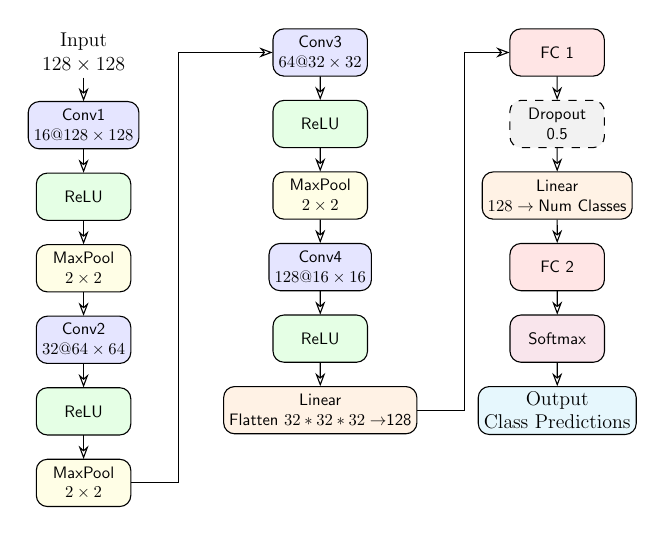
\begin{tikzpicture}[
        font=\sffamily,
        node distance=0.5cm and 1.5cm,
        scale=0.6,
        transform shape,
        >={Stealth[open]},
        every node/.style={align=center},
        conv/.style={draw, minimum width=2cm, minimum height=1cm, rounded corners, fill=blue!10},
        relu/.style={draw, minimum width=2cm, minimum height=1cm, rounded corners, fill=green!10},
        pool/.style={draw, minimum width=2cm, minimum height=1cm, rounded corners, fill=yellow!10},
        linear/.style={draw, minimum width=2cm, minimum height=1cm, rounded corners, fill=orange!10},
        fc/.style={draw, minimum width=2cm, minimum height=1cm, rounded corners, fill=red!10},
        drop/.style={draw, dashed, minimum width=2cm, minimum height=1cm, rounded corners, fill=gray!10},
        softmax/.style={draw, minimum width=2cm, minimum height=1cm, rounded corners, fill=purple!10},
        input/.style={font=\large},
        output/.style={draw, minimum width=2cm, minimum height=1cm, rounded corners, fill=cyan!10, font=\large}
    ]
    \node[input] (input) {Input \\ $128 \times 128$};
    \node[conv, below=of input] (conv1) {Conv1 \\ $16@128 \times 128$};
    \node[relu, below=of conv1] (relu1) {ReLU};
    \node[pool, below=of relu1] (pool1) {MaxPool \\ $2\times 2$};
    \node[conv, below=of pool1] (conv2) {Conv2 \\ $32@64 \times 64$};
    \node[relu, below=of conv2] (relu2) {ReLU};
    \node[pool, below=of relu2] (pool2) {MaxPool \\ $2\times 2$};
    
    \node[conv, right=3cm of input] (conv3) {Conv3 \\ $64@32 \times 32$};
    \node[relu, below=of conv3] (relu3) {ReLU};
    \node[pool, below=of relu3] (pool3) {MaxPool \\ $2\times 2$};
    \node[conv, below=of pool3] (conv4) {Conv4 \\ $128@16 \times 16$};
    \node[relu, below=of conv4] (relu4) {ReLU};
    \node[linear, below=of relu4] (linear1) {Linear \\ Flatten $32*32*32 \to $128};

    \node[fc, right=3cm of conv3] (fc1) {FC 1};
    \node[drop, below=of fc1] (drop1) {Dropout \\ 0.5};
    \node[linear, below=of drop1] (linear2) {Linear \\ $128 \to \text{Num Classes}$};
    \node[fc, below=of linear2] (fc2) {FC 2};
    \node[softmax, below=of fc2] (softmax) {Softmax};
    \node[output, below=of softmax] (output) {Output \\ Class Predictions};

    \draw[->] (input.south) -- (conv1.north);
    \draw[->] (conv1.south) -- (relu1.north);
    \draw[->] (relu1.south) -- (pool1.north);
    \draw[->] (pool1.south) -- (conv2.north);
    \draw[->] (conv2.south) -- (relu2.north);
    \draw[->] (relu2.south) -- (pool2.north);
    \draw[->] (pool2.east) -- ++(1.0,0) |- (conv3.west);
    \draw[->] (conv3.south) -- (relu3.north);
    \draw[->] (relu3.south) -- (pool3.north);
    \draw[->] (pool3.south) -- (conv4.north);
    \draw[->] (conv4.south) -- (relu4.north);
    \draw[->] (relu4.south) -- (linear1.north);

    \draw[->] (linear1.east) -- ++(1.0,0) |- (fc1.west);
    \draw[->] (fc1.south) -- (drop1.north);
    \draw[->] (drop1.south) -- (linear2.north);
    \draw[->] (linear2.south) -- (fc2.north);
    \draw[->] (fc2.south) -- (softmax.north);
    \draw[->] (softmax.south) -- (output.north);

    \end{tikzpicture}
    \caption{Forward Pass of the CNN Model used for the Open and Closed Set Identification.}
    \label{fig:model-1}
\end{figure}

\begin{figure}[h!]
    \centering
    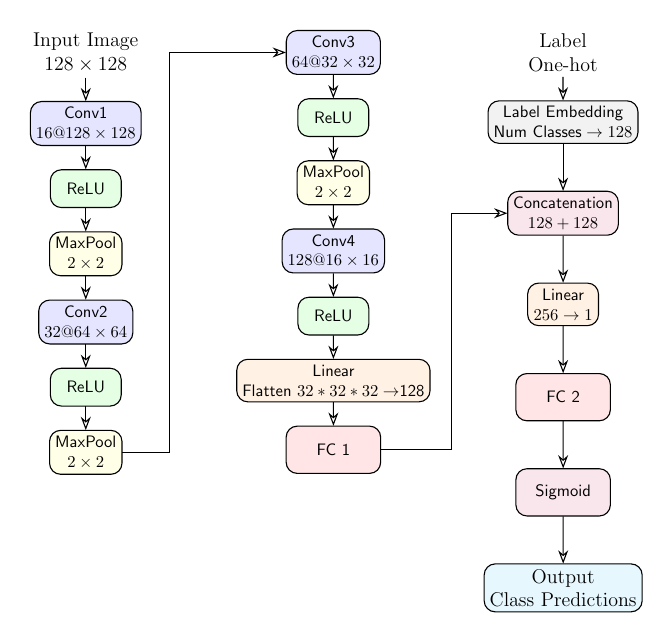
\begin{tikzpicture}[
        font=\sffamily,
        node distance=0.5cm and 1.5cm,
        scale=0.6,
        transform shape,
        >={Stealth[open]},
        every node/.style={align=center},
        conv/.style={draw, minimum width=1.5cm, minimum height=0.8cm, rounded corners, fill=blue!10},
        relu/.style={draw, minimum width=1.5cm, minimum height=0.8cm, rounded corners, fill=green!10},
        pool/.style={draw, minimum width=1.5cm, minimum height=0.8cm, rounded corners, fill=yellow!10},
        embed/.style={draw, minimum width=1.5cm, minimum height=0.8cm, rounded corners, fill=gray!10},
        fc/.style={draw, minimum width=2cm, minimum height=1cm, rounded corners, fill=red!10},
        linear/.style={draw, minimum width=1.5cm, minimum height=0.8cm, rounded corners, fill=orange!10},
        concat/.style={draw, minimum width=1.5cm, minimum height=0.8cm, rounded corners, fill=purple!10},
        sigmoid/.style={draw, minimum width=2cm, minimum height=1cm, rounded corners, fill=purple!10},
        input/.style={font=\large},
        output/.style={draw, minimum width=1.5cm, minimum height=0.8cm, rounded corners, fill=cyan!10, font=\large}
    ]
    \node[input] (image_input) {Input Image \\ $128 \times 128$};
    \node[conv, below=of image_input] (conv1) {Conv1 \\ $16@128 \times 128$};
    \node[relu, below=of conv1] (relu1) {ReLU};
    \node[pool, below=of relu1] (pool1) {MaxPool \\ $2\times 2$};
    \node[conv, below=of pool1] (conv2) {Conv2 \\ $32@64 \times 64$};
    \node[relu, below=of conv2] (relu2) {ReLU};
    \node[pool, below=of relu2] (pool2) {MaxPool \\ $2\times 2$};
    \node[conv, right=3cm of image_input] (conv3) {Conv3 \\ $64@32 \times 32$};
    \node[relu, below=of conv3] (relu3) {ReLU};
    \node[pool, below=of relu3] (pool3) {MaxPool \\ $2\times 2$};
    \node[conv, below=of pool3] (conv4) {Conv4 \\ $128@16 \times 16$};
    \node[relu, below=of conv4] (relu4) {ReLU};
    \node[linear, below=of relu4] (linear1) {Linear \\ Flatten $32*32*32 \to $128};
    \node[fc, below=of linear1] (fc_image) {FC 1};
    \node[input, right=3cm of conv3] (label_input) {Label \\ One-hot};
    \node[embed, below=of label_input] (label_embed) {Label Embedding \\ $\text{Num Classes} \to 128$};
    \node[concat, below=of label_embed, yshift=-0.5cm] (concat) {Concatenation \\ $128 + 128$};
    \node[linear, below=of concat, yshift=-0.5cm] (linear2) {Linear \\ $256 \to 1$};
    \node[fc, below=of linear2, yshift=-0.5cm] (fc_final) {FC 2};
    \node[sigmoid, below=of fc_final, yshift=-0.5cm] (sigmoid) {Sigmoid};
    \node[output, below=of sigmoid, yshift=-0.5cm] (output) {Output \\ Class Predictions};

    \draw[->] (image_input.south) -- (conv1.north);
    \draw[->] (conv1.south) -- (relu1.north);
    \draw[->] (relu1.south) -- (pool1.north);
    \draw[->] (pool1.south) -- (conv2.north);
    \draw[->] (conv2.south) -- (relu2.north);
    \draw[->] (relu2.south) -- (pool2.north);
    \draw[->] (pool2.east) -- ++(1.0,0) |- (conv3.west);
    \draw[->] (conv3.south) -- (relu3.north);
    \draw[->] (relu3.south) -- (pool3.north);
    \draw[->] (pool3.south) -- (conv4.north);
    \draw[->] (conv4.south) -- (relu4.north);
    \draw[->] (relu4.south) -- (linear1.north);
    \draw[->] (linear1.south) -- (fc_image.north);
    \draw[->] (label_input.south) -- (label_embed.north);
    \draw[->] (fc_image.east) -- ++(1.5,0) |- (concat.west);
    \draw[->] (label_embed.south) -- ++(0,-0.8) -| (concat.north);
    \draw[->] (concat.south) -- (linear2.north);
    \draw[->] (linear2.south) -- (fc_final.north);
    \draw[->] (fc_final.south) -- (sigmoid.north);
    \draw[->] (sigmoid.south) -- (output.north);

    \end{tikzpicture}
    \caption{Forward Pass of the CNN Model used for Verification.}
    \label{fig:model-2}
\end{figure}

\textbf{Model 2} The CNN Model Architecture presented in Figure \ref{fig:model-2} is used for Verification. Designed with the goal of verifiying the authenticity of a given image-label pair, this model uses a shared backbone to extract features from the input image. The model then uses a linear layer to extract a compact feature representation, followed by label embeddings to capture label-specific information. It concatenates the 128-dimensional image features with the label embeddings to form a combined 256-dimensional vector. This fused representation is passed through a fully connected layer and sigmoid activation to output a verification score between 0 and 1.

\tikzset{
startstop/.style={rectangle, rounded corners, minimum width=2.5cm, minimum height=0.8cm, text centered, draw=black, fill=red!30},
process/.style={rectangle, minimum width=2.5cm, minimum height=0.8cm, text centered, draw=black, fill=blue!30},
decision/.style={diamond, minimum width=2.5cm, minimum height=0.8cm, text centered, draw=black, fill=green!30},
evaluation/.style={rectangle, rounded corners=0.2cm, minimum width=2.5cm, minimum height=0.8cm, text centered, draw=black, fill=yellow!50},
roundmodel/.style={circle, minimum size=2.0cm, text centered, draw=black, fill=gray!50},
flatgreen/.style={rectangle, rounded corners, minimum width=2.5cm, minimum height=0.8cm, text centered, draw=black, fill=green!50},
purpleblock/.style={rectangle, rounded corners, minimum width=2.5cm, minimum height=0.8cm, text centered, draw=black, fill=purple!50},
arrow/.style={thick,->,>=stealth}
}

\section{Experimental}
This section describes the experimental setup introducing the 3 evaluation setups used to assess the performance of the proposed biometric system and the data splitting strategy used for each evaluation setup.

\subsection{Evaluation Setups}
The evaluation was performed using three distinct types of evaluations:

\begin{itemize}
    \item \textbf{Identification with a Closed Set}: involves including all enrolled patients in the dataset. Each image is classified into one of the known classes (patients) based on its extracted features. The system is trained and tested with the same predefined set of enrolled patients, ensuring no unknown users are present in the dataset.

    \item \textbf{Identification with an Open Set}: excludes a percentage of the enrolled patients from the dataset during training. These excluded patients represent unknown users during the evaluation phase. The model is tested on both known and unknown classes, where the unknown classes are expected to be classified as unknown to simulate open-set identification.

    \item \textbf{Verification}: tests the system's ability to verify the identity of users. Genuine samples consist of images correctly matched to their claimed identities, while imposter samples are created by associating images with incorrect user identities to simulate attempts to mislead the system.
\end{itemize}

\begin{figure}[!ht]
    \centering
    \resizebox{0.56\columnwidth}{!}{
    \begin{tikzpicture}[node distance=1.8cm]
    \node (input) [startstop] {\includegraphics[width=2.5cm]{./images/preprocessing/selected_image.jpg}};
    \node (preprocess) [process, below of=input, yshift=-0.5cm] {Preprocessing};
    \node (binary) [purpleblock, below of=preprocess, yshift=-0.5cm] {\includegraphics[width=2.5cm]{./images/preprocessing/binarize_image.png}};
    \node (open) [evaluation, below left of=binary, xshift=-2cm, yshift=-1.5cm] {Identification Open};
    \node (closed) [evaluation, below of=binary, yshift=-2cm] {Identification Closed};
    \node (verify) [evaluation, below right of=binary, xshift=2cm, yshift=-1.5cm] {Verification};
    \node (claimed) [startstop, above of=verify, yshift=2cm] {Claimed Identity};
    \node (cnn) [roundmodel, below of=closed, yshift=-1.0cm] {CNN Model};
    \node (output) [flatgreen, below of=cnn, yshift=-0.3cm] {Prediction};
    \draw [arrow] (input) -- (preprocess);
    \draw [arrow] (preprocess) -- (binary);
    \draw [arrow] (binary) -- (open);
    \draw [arrow] (binary) -- (closed);
    \draw [arrow] (binary) -- (verify);
    \draw [arrow] (verify) -- (cnn);
    \draw [arrow] (claimed) -- (verify);
    \draw [arrow] (open) -- (cnn);
    \draw [arrow] (closed) -- (cnn);
    \draw [arrow] (cnn) -- (output);
    \end{tikzpicture}%
    }
    \caption{Experimental Pipeline}
\end{figure}

\newpage

\subsection{Data Splitting}
To ensure consistent data processing, only images of the left hand were selected from the dataset. This decision was based on the observation that left-hand images generally show fewer imperfections, such as skin damages, which could introduce variability and noise. Additionally, the 850 nm spectrum was chosen for image acquisition. This wavelength was selected because it primarily captures palm vein patterns, avoiding interference from extraneous details such as palm lines that are more visible at the 940 nm spectrum.

The dataset used in this study was split differently for the three evaluation setups:

\textbf{Identification with a Closed Set} includes all patients in the dataset, and their images are divided into training and test sets. The first four images per patient are used for training and the remaining 2 images are used for testing. This setup ensures that all enrolled patients contribute images to the training and testing phases, facilitating evaluation in a controlled, closed-set scenario.

\textbf{Identification with an Open Set} 70\% of patients are randomly selected as known, with their images split into training (first four images) and testing (remaining 2 images). The remaining 30\% serve as unknown patients, with their images used solely for testing to assess the system's ability to handle unenrolled users. 

\textbf{Verification} includes genuine and imposter samples for evaluation. For each patient, the first four images are used for training, and the remaining 2 images are used for testing. Genuine samples consist of matching the correct image to the claimed identity, while imposter samples are created by pairing images from different patients, simulating attempts to impersonate other users. 

To ensure consistency and reproducibility across all splits, a fixed random seed was used during shuffling. This guarantees that the data partitioning remains consistent across different runs and experiments.
\section{Evaluation Metrics}
The evaluation metrics used to measure the performance of the Biometric Systems in the 3 experimental scenarios are liste below.

\begin{itemize}

    \item \textbf{False Acceptance Rate (FAR)}:  
    Percentage of impostor samples incorrectly accepted by the system.  
    \[
    \text{FAR} = \frac{\text{Number of False Acceptances}}{\text{Total Number of Attempts}} \times 100
    \]
    Lower FAR values indicate a more secure system while a higher FAR signifies a higher risk of impostor acceptance.
    
    \item \textbf{False Rejection Rate (FRR)}:  
    Percentage of genuine samples incorrectly rejected by the system.  
    \[
    \text{FRR} = \frac{\text{Number of False Rejections}}{\text{Total Number of Attempts}} \times 100
    \]
    Lower FRR values indicate a more reliable system while a higher FRR signifies a higher risk of genuine rejection.

    \item \textbf{Equal Error Rate (EER)}:  
    The point where the FAR and FRR are equal, providing a single measure of system performance.  
    A lower EER signifies a more balanced system.

    \item \textbf{Receiver Operating Characteristic (ROC) Curve}:  
    Curve plotted on a Cartesian plane where the axes are Genuine Acceptance Rate and False Acceptance Rate. It represents the probability of correctly identifying a subject as the FAR varies.

    \item \textbf{Detection Error Tradeoff (DET) Curve}:  
    A variation of the ROC curve that plots the FRR against the FAR on a logarithmic scale, providing insight into trade-offs between errors.

    \item \textbf{Cumulative Match Characteristic (CMC) Curve}:  
    Represents the probability of correct identification as a function of rank in a closed-set scenario. Higher Rank-1 and rapid convergence to 1.0 indicate strong identification performance.

    \item \textbf{Confusion Matrix}:  
    The confusion matrix is a tool used to evaluate the performance of a classification model. It consists of a table where the columns are Predicted Negative and Predicted Positive, while the rows are Real Negative and Real Positive, comparing the model's predictions with the actual classes of the dataset. Below is a generic representation of a confusion matrix:
    \[
    \begin{array}{c|c|c}
          & \text{PN} & \text{PP} \\ \hline
        \text{RN} & \text{TN} & \text{FP} \\ 
        \text{RP} & \text{FN} & \text{TP} \\
    \end{array}
    \]
  
    \begin{itemize}
        \item \textbf{FP (False Positive)}:  
        The model incorrectly predicted that an instance belongs to the positive class when it actually belongs to the negative class (false alarm).
        
        \item \textbf{FN (False Negative)}:  
        The model incorrectly predicted that an instance belongs to the negative class when it actually belongs to the positive class (missed detection).
        
        \item \textbf{TN (True Negative)}:  
        The model correctly predicted that an instance belongs to the negative class.
        
        \item \textbf{TP (True Positive)}:  
        The model correctly predicted that an instance belongs to the positive class.
    \end{itemize}

    \item \textbf{Open-set (Watchlist) Receiver Operating Characteristic (ROC)}: Depicts DIR against FAR and is useful for finding the optimal threshold, balancing the maximization of DIR and the minimization of FAR. A compromise is necessary as both measures depend on the threshold, but in opposite directions:
    \begin{itemize}
        \item If we raise the threshold, FAR decreases, but DIR also decreases.
        \item If we lower the threshold, DIR increases, but FAR also increases.
    \end{itemize}

\end{itemize}

\section{Results}
The results of the evaluation metrics for the Biometric Systems in the 3 experimental scenarios are presented below with comments on the performance of the systems.

\subsection{Identification with a Closed Set}

The biometric system's performance for closed-set identification was evaluated using the Cumulative Match Characteristic (CMC) curve, which measures the probability of correct identification at various ranks.

\begin{figure}[!ht]
    \centering
    \includegraphics[width=\columnwidth]{./images/plots/id-close/cmc_curve.png}
    \caption{CMC Curve demonstrating the probability of identification across ranks for closed-set identification.}
    \label{fig:cmc_curve}
\end{figure}

\textbf{CMC Curve}: The CMC curve indicates that the system achieves a Rank-1 identification rate of 83.50\%, highlighting its ability to correctly identify subjects in the top rank most of the time. The curve rapidly approaches a probability of 1.0 as the rank increases.

\subsection{Identification with an Open Set}

The biometric system's performance for open-set identification was evaluated using the Watchlist Receiver Operating Characteristic (ROC) curve, plotting the Detection and Identification Rate (DIR) against the False Alarm Rate (FAR).

\begin{figure}[!ht]
    \centering
    \includegraphics[width=\columnwidth]{./images/plots/id-open/watchlist_roc_curve.png}
    \caption{Watchlist ROC Curve demonstrating the DIR vs. FAR for open-set identification.}
    \label{fig:watchlist_roc_curve}
\end{figure}

\textbf{Watchlist ROC Curve}: The ROC curve demonstrates the system's effectiveness in maintaining a high Detection and Identification Rate (DIR) while minimizing the False Alarm Rate (FAR). The curve achieves strong performance, as evidenced by a consistent increase in DIR with lower FAR values. Threshold markers along the curve provide insights into the system's operating characteristics and trade-offs between detection and false alarms. 

\subsection{Verification}

The biometric verification system was evaluated using False Acceptance Rate (FAR), False Rejection Rate (FRR), Equal Error Rate (EER), Receiver Operating Characteristic (ROC) and Detection Error Tradeoff (DET) curves, and a Confusion Matrix to assess the system's performance.

\begin{figure}[!ht]
    \centering
    \begin{subfigure}[t]{0.48\columnwidth}
        \includegraphics[width=\textwidth]{./images/plots/ver/far_vs_frr.png}
        \caption{FAR vs. FRR}
        \label{fig:far_vs_frr}
    \end{subfigure}
    \hfill
    \begin{subfigure}[t]{0.48\columnwidth}
        \includegraphics[width=\textwidth]{./images/plots/ver/confusion_matrix.png}
        \caption{Confusion Matrix}
        \label{fig:confusion_matrix}
    \end{subfigure}
\end{figure}

\textbf{FAR vs. FRR Analysis}: The FAR and FRR curves intersect at a threshold of 0.5025, yielding an EER of 0.5025. This indicates a balanced trade-off between the acceptance of impostors and rejection of genuine users, critical for assessing verification performance.

\textbf{Confusion Matrix}: The system achieved a good balance between true positives (158) and true negatives (153) while maintaining acceptable rates of false positives (42) and false negatives (46).

\begin{figure}[!ht]
    \centering
    \begin{subfigure}[t]{0.48\columnwidth}
        \includegraphics[width=\textwidth]{./images/plots/ver/roc_curve.png}
        \caption{ROC Curve}
        \label{fig:roc_curve}
    \end{subfigure}
    \hfill
    \begin{subfigure}[t]{0.48\columnwidth}
        \includegraphics[width=\textwidth]{./images/plots/ver/det_curve.png}
        \caption{DET Curve}
        \label{fig:det_curve}
    \end{subfigure}
\end{figure}

\textbf{ROC Curve}: With an Area Under the Curve (AUC) of 0.8671, the ROC curve demonstrates strong discriminatory power between genuine and impostor samples.

\textbf{Detection Error Tradeoff (DET) Curve}: The DET curve highlights the system's error rates over a range of operating conditions. The downward trend reflects the system's ability to minimize errors as the threshold is optimized.
\section{Conclusion and Future Work}
\subsection{Conclusion}

In this work, a straightforward yet highly effective CNN-based recognition system was developed for the purpose of hand vein recognition. Despite the architecture's simplicity, it demonostrated remarkable efficiency by achieving rapid training convergence and maintaining low computational requirements. The results indicate that the model achieves an accuracy of \textbf{xx.x\%} on the training set, traslating to a robust perfomance when deployed on the test set, where it obtained an accuracy of \textbf{xx.x\%}. Such a perfomance level is significant for a recognition task, as it ensures reliable identification while keeping resource consumption and development complexity to a minimum. Overall, this implementation highlights that even a relatively uncomplicated CNN framework can deliver strong accuracy and efficiency, making it an appealing solution for practical vein-based recognition systems.

\subsection{Future Work}

An interesting extension to this project for future exploration involves expanding the focus beyond the current palm-based Region of Interest (ROI). Instead of restricting the system solely to the palm vein pattern, it would be beneficial to consider additional hand characteristics such as overall hand geometry, finger length and spacing, and other distinctive biometric features of the hand. Using these complementary features would allow us to develop multiple specialized models, one dedicated to palm veins (as implemented in this project), another concentrating on hand geometry, another on finger structure, and so on. By utilizing an ensemble learning strategy (see Figure~\ref{fig:ensemble}), where each specialized model contributes its prediction, we could combine these outputs into a final, more robust decision. This multi-model, ensemble-based approach has the potential to significantly improve the overall accuracy and reliability of the system.

\begin{figure}[h]
    \centering
    \resizebox{0.4\textwidth}{!}{% Scale reduced to 40% of text width
        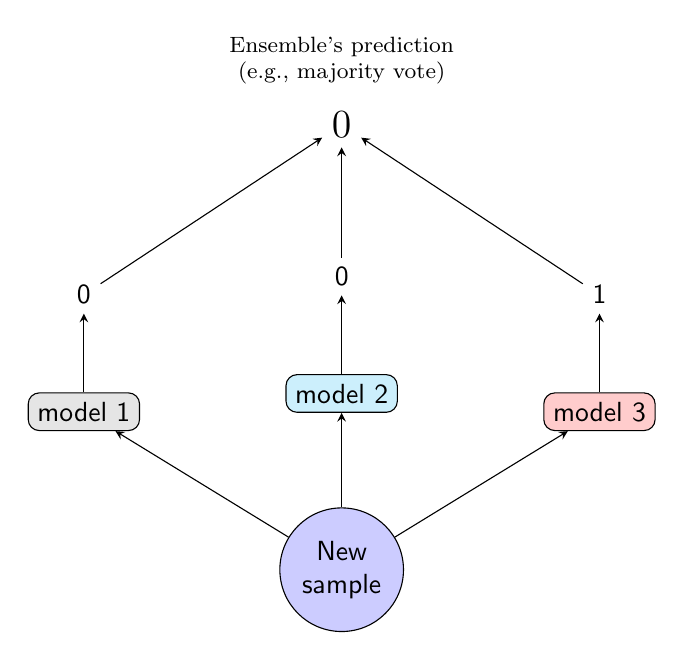
\begin{tikzpicture}[
            font=\sffamily,
            >=stealth,
            node distance=1cm,
            every node/.style={align=center}
        ]
            \node[circle, draw, fill=blue!20, minimum size=1cm] (sample) {New\\sample};

            \node[rectangle, draw, rounded corners, fill=gray!20, 
                  above left=1.2cm and 2cm of sample] (model1) {model 1};
            \node[rectangle, draw, rounded corners, fill=cyan!20, 
                  above=1.2cm of sample] (model2) {model 2};
            \node[rectangle, draw, rounded corners, fill=red!20, 
                  above right=1.2cm and 2cm of sample] (model3) {model 3};

            \node[above=1.0cm of model1] (pred1) {0};
            \node[above=1.0cm of model2] (pred2) {0};
            \node[above=1.0cm of model3] (pred3) {1};

            \node[above=1.4cm of pred2, font=\Large] (ens) {0};
            \node[font=\footnotesize, above=3pt of ens] (ensLabel) 
                 {Ensemble’s prediction\\(e.g., majority vote)};

            \draw [->] (sample) -- (model1);
            \draw [->] (sample) -- (model2);
            \draw [->] (sample) -- (model3);

            \draw [->] (model1) -- (pred1);
            \draw [->] (model2) -- (pred2);
            \draw [->] (model3) -- (pred3);

            \draw [->] (pred1) -- (ens);
            \draw [->] (pred2) -- (ens);
            \draw [->] (pred3) -- (ens);

        \end{tikzpicture}
    } % End of resizebox
    \caption{Illustration of an ensemble learning strategy. Each model processes the same input and produces a prediction. These predictions are combined (e.g., through majority voting) to create the ensemble's final output.}
    \label{fig:ensemble}
\end{figure}

\bibliographystyle{apalike} 
\bibliography{bibliography.bib}

\end{document}